\section{Results}
\label{sec:results}

%% FIGURE: Visual comparison of controller performance for the block M.
\begin{figure*}
    \centering
    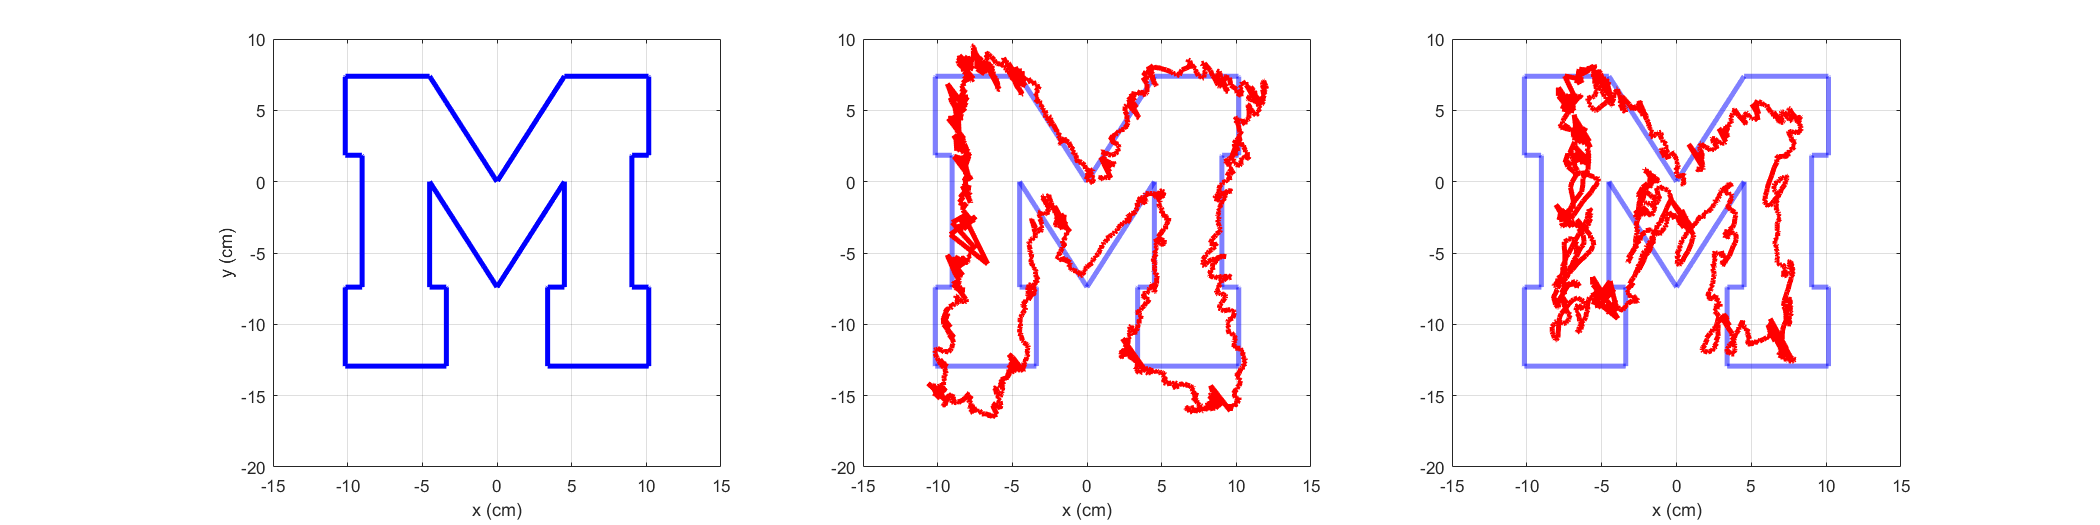
\includegraphics[width=\linewidth]{figures/compare_blockM_300s_draft.png}
    \caption{Reference trajectory (left). MPC with Koopman model (middle). MPC with linear model (right)}
    \label{fig:compare_blockM}
\end{figure*}

%% FIGURE: Visual comparison of controller performance for the pacman.
\begin{figure*}
    \centering
    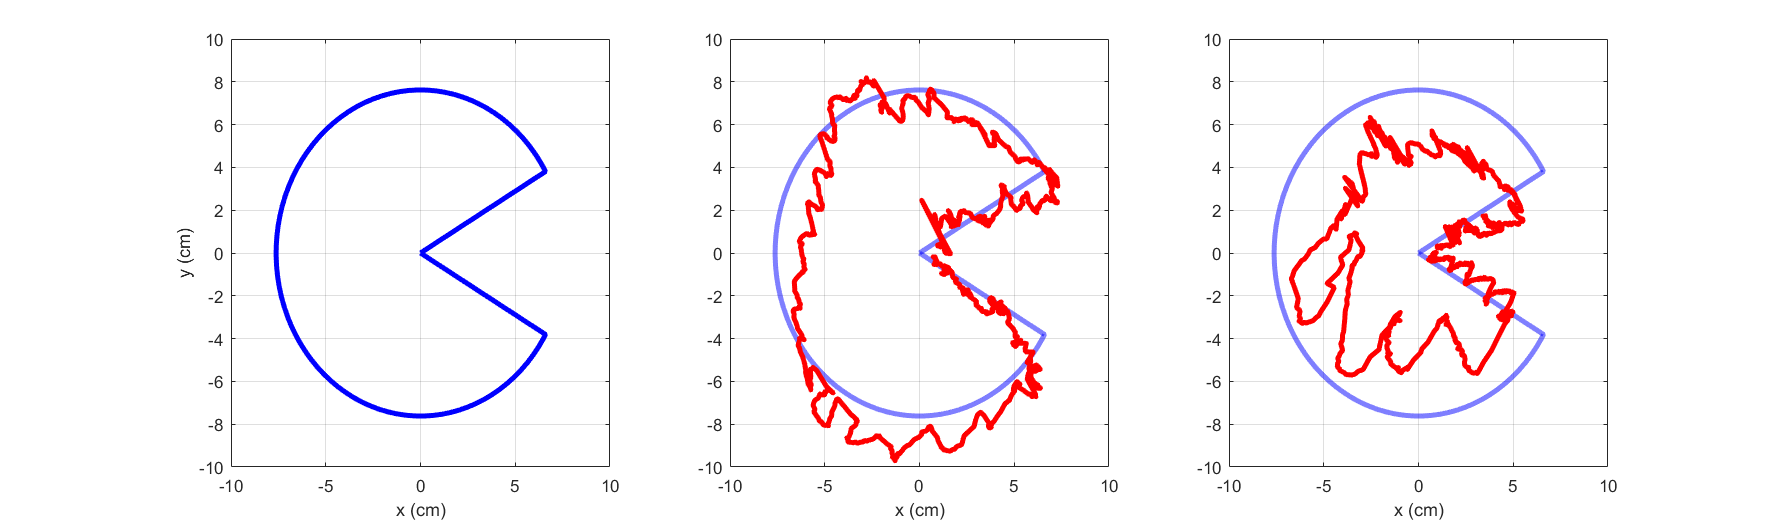
\includegraphics[width=\linewidth]{figures/compare_pacman68_90s_draft.png}
    \caption{Reference trajectory (left). MPC with Koopman model (middle). MPC with linear model (right)}
    \label{fig:compare_pacman}
\end{figure*}

%% TABLE: RMSE results table
\begin{table}[]
    \rowcolors{2}{white}{gray!25}
    \setlength\tabcolsep{5pt} % default value: 6pt
    \centering
    \caption{RMSE (cm) over all trajectory following tasks \Dan{Fill in real results later}}
    \begin{tabular}{|c|c|c|c|c|c|c|c|c|}
        \hline
        \rowcolor{white} 
        & \multicolumn{6}{c |}{\textbf{States}} & & \textbf{Std.} \\
        \cline{2-7} \rowcolor{white}
        \multirow{-2}{*}{\textbf{Model}} & $x_1$ & $x_2$ & $x_3$ & $x_4$ & $x_5$ & $x_6$ & \multirow{-2}{*}{\textbf{Avg.}} & \textbf{Dev.} \\
        \hline
        % RESULTS FOR ROBOT A
        Koopman     &  2.4  &  2.0  &  2.9  &  1.7  &  1.5  &  2.0 & 2.1 & 0.5 \\
        Neural Net  &  5.8  &  4.0  &  6.6  &  3.9  &  2.8  &  3.5 & 4.5 & 1.5 \\
        State Space &  5.1  &  3.1  &  9.9  &  3.0  &  1.8  &  4.8 & 4.6 & 2.9 \\
        Ham.-Weiner &  7.0  &  4.5  &  6.9  &  3.0  &  2.3  &  3.1 & 4.5 & 2.0 \\
        % \multirow{-5}{*}{\cellcolor{white} \rotatebox[origin=c]{90}{\textbf{Robot A}}}
        NLARX       &  5.0  &  3.0 &  12.0  &  3.8  &  2.1  &  2.8 & 4.8 & 3.7 \\
        \hline
        % % RESULTS FOR ROBOT B
        % \cellcolor{white} & Koopman & & & & & & & & \\
        % \cellcolor{white} & Neural Net & & & & & & & & \\
        % \cellcolor{white} & State Space & & & & & & & & \\
        % \cellcolor{white} & Ham.-Weiner & & & & & & & & \\
        % \multirow{-5}{*}{\cellcolor{white} \rotatebox[origin=c]{90}{\textbf{Robot B}}}
        % & NLARX & & & & & & & & \\
        % \hline
    \end{tabular}
    \label{tab:RMSE}
\end{table}
